\documentclass[a4paper,11pt]{article}
\usepackage[left=2cm,text={17cm, 24cm},top=3cm]{geometry}
\usepackage[czech]{babel}
\usepackage{times}
\usepackage[utf8]{inputenc}
\usepackage[unicode]{hyperref}
\usepackage{changepage}
\usepackage{amsthm, amssymb, amsmath}

\usepackage{graphics}
\usepackage{pdflscape}
\usepackage{multirow}
\usepackage{algorithmic}
\usepackage[ruled,vlined,czech]{algorithm2e}


\begin{document}

\begin{titlepage}
\begin{center}
\Huge
\textsc{Vysoké učení technické v Brně}\\
\textsc{Fakulta informačních technologií}\\
\vspace{\stretch{0.382}}
\huge
Typografie a publikování\,--\,3. projekt\\
\Huge
Tabulky a obrázky\\
\vspace{\stretch{0.618}}
\end{center}
{\LARGE \today \hfill Martin Litwora}
\end{titlepage}


\section{Úvodní strana}
Název práce umístěte do zlatého řezu a nezapomeňte uvést dnešní datum a vaše jméno a příjmení.

\section{Tabulky}
Pro sázení tabulek můžeme použít buď prostředí \texttt{tabbing} nebo prostředí \texttt{tabular}.

\subsection{Prostředí \texttt{tabbing}}
Při použití \texttt{tabbing} vypadá tabulka následovně:
\begin{tabbing}
\textbf{Ovoce}  \qquad \qquad \ \= \textbf{Cena} \quad \= \textbf{Množství} \\
Jablka \> 25,90 \> 3 kg \\
Hrušky \> 27,40 \> 2,5kg\\
Vodní melouny \> 35,-- \> 1 kus
\end{tabbing}
Toto prostředí se dá také použít pro sázení algoritmů, ovšem vhodnější je použít prostředí \texttt{algorithm} nebo \texttt{algorithm2e} (viz sekce \ref{algoritmy}).

\subsection{Prostředí \texttt{tabular}}
Další možností, jak vytvořit tabulku, je použít prostředí \texttt{tabular}. Tabulky pak budou vypadat takto\footnote{Kdyby byl problém s \texttt{cline}, zkuste se podívat třeba sem: \url{http://www.abclinuxu.cz/tex/poradna/show/325037}.}:

\begin{table}[h]
    \catcode`\-=12 % kvuli cline
    \centering
    \begin{tabular}{|c|c|c|}
    \hline
     & \multicolumn{2}{ c|}{\textbf{Cena}} \\
     \cline{2-3}
        \textbf{Měna} & \textbf{nákup} & \textbf{prodej} \\
        \hline
        EUR & 25,475 & 27,045 \\
        GBP & 28,835 & 30,705 \\
        USD & 22,943 & 24,357 \\
    \hline
    \end{tabular}
    \caption{Tabulka kurzů k dnešnímu dni}
    \label{tab1}
\end{table}

\begin{table}[h]
    \centering
    \catcode`\-=12 % kvuli cline
    \begin{tabular}{|c|c|}
    \hline
        $A$ & $\neg A$ \\
        \hline
        \textbf{P} & N \\
        \hline
        \textbf{O} & O \\
        \hline
        \textbf{X} & X \\
        \hline
        \textbf{N} & P \\
        \hline
    \end{tabular}
    \begin{tabular}{|c|c|c|c|c|c|}
    \hline
        \multicolumn{2}{|c|}{\multirow{2}{*}{$A \wedge B$}} & \multicolumn{4}{c|}{$B$} \\
        \cline{3-6}
        \multicolumn{2}{|c|}{} & \textbf{P} & \textbf{O} & \textbf{X} & \textbf{N} \\
        \hline
        \multirow{4}{*}{$A$} & \textbf{P} & P & O & X & N \\
        \cline{2-6}
         & \textbf{O} & O & O & N & N \\
        \cline{2-6}
         & \textbf{X} & X & N & X & N \\
        \cline{2-6}
         & \textbf{N} & N & N & N & N \\
        \hline
    \end{tabular}
    \begin{tabular}{|c|c|c|c|c|c|}
    \hline
        \multicolumn{2}{|c|}{\multirow{2}{*}{$A \vee B$}} & \multicolumn{4}{c|}{$B$} \\
        \cline{3-6}
        \multicolumn{2}{|c|}{} & \textbf{P} & \textbf{O} & \textbf{X} & \textbf{N} \\
        \hline
        \multirow{4}{*}{$A$} & \textbf{P} & P & P & P & P \\
        \cline{2-6}
         & \textbf{O} & P & O & P & O \\
        \cline{2-6}
         & \textbf{X} & P & P & X & X \\
        \cline{2-6}
         & \textbf{N} & P & O & X & N \\
        \hline
    \end{tabular}
    \begin{tabular}{|c|c|c|c|c|c|}
    \hline
        \multicolumn{2}{|c|}{\multirow{2}{*}{$A \rightarrow B$}} & \multicolumn{4}{c|}{$B$} \\
        \cline{3-6}
        \multicolumn{2}{|c|}{} & \textbf{P} & \textbf{O} & \textbf{X} & \textbf{N} \\
        \hline
        \multirow{4}{*}{$A$} & \textbf{P} & P & O & X & N \\
        \cline{2-6}
         & \textbf{O} & P & O & P & O \\
        \cline{2-6}
         & \textbf{X} & P & P & X & X \\
        \cline{2-6}
         & \textbf{N} & P & P & P & P \\
        \hline
    \end{tabular}
    \caption{Protože Kleeneho trojhodnotová logika už je \uv{zastaralá}, uvádíme si zde příklad čtyřhodnotové logiky}
    \label{tab2}
\end{table}
\newpage

\section{Algoritmy} \label{algoritmy}
Pokud budeme chtít vysázet algoritmus, můžeme použít prostředí \texttt{ algorithm}\footnote{Pro 	nápovědu, jak zacházet s prostředím \texttt{algorithm}, můžeme zkusit tuhle stránku: \\ \url{http://ftp.cstug.cz/pub/tex/CTAN/macros/latex/contrib/algorithms/algorithms.pdf}.} \ nebo \texttt{ algorithm2e}\footnote{Pro algorithm2e zase tuhle: \url{http://ftp.cstug.cz/pub/tex/CTAN/macros/latex/contrib/algorithm2e/doc/algorithm2e.pdf}.}. Příklad použití prostředí \texttt{algorithm2e} viz Algoritmus \ref{alg1}.

\begin{algorithm}
\caption{\textsc{FastSLAM}}
\label{alg1}
\textbf{Input:} $(X_{t-1},u_t,z_t)$ \\
\textbf{Output:} $X_t$
\medskip
\algsetup{indent=2em}
\begin{algorithmic}[1]
\STATE $\overline{X_t} = X_t = 0$
\FOR{$k = 1$ to $M$}
\STATE $x_t^{[k]} = $ \textit{sample\_motion\_model}$(u_t,x_{t-1}^{[k]})$
\STATE $\omega _t^{[k]} = $ \textit{measurement\_model}$(z_t,x_t^{[k]},m_{t-1})$
\STATE $m_t^{[k]} = $ \textit{updated\_occupancy\_grid}$(z_t,x_t^{[k]},m_{t-1}^{[k]})$
\STATE $\overline{X_t} = \overline{X_t} + \langle x_x^{[m]},\omega _t^{[m]} \rangle$
\ENDFOR
\FOR{$k = 1$ to $M$}
\STATE draw $i$ with probability $\approx \omega _t^{[i]}$
\STATE add $\langle x_x^{[k]},m_t^{[k]} \rangle$ to $X_t$
\ENDFOR
\RETURN $X_t$
\end{algorithmic}
\end{algorithm}

\section{Obrázky}
Do našich článků můžeme samozřejmě vkládat obrázky. Pokud je obrázkem fotografie, můžeme klidně použít bitmapový soubor. Pokud by to ale mělo být nějaké schéma nebo něco podobného, je dobrým zvykem takovýto obrázek vytvořit vektorově.

\begin{figure}[h]
    \centering
    \scalebox{0.4}{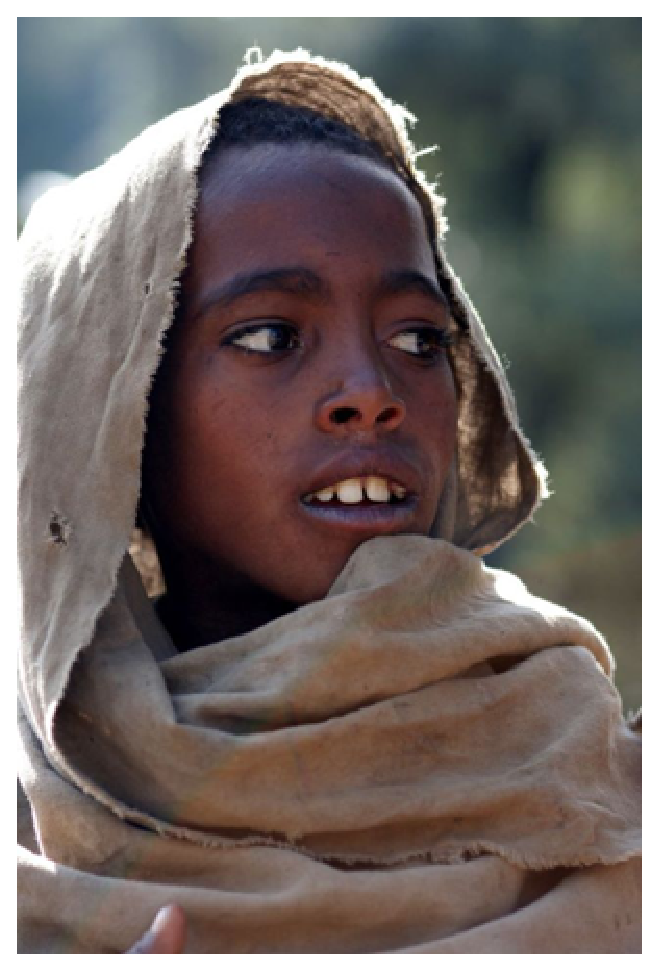
\includegraphics{etiopan.eps}}
    \reflectbox{\scalebox{0.4}{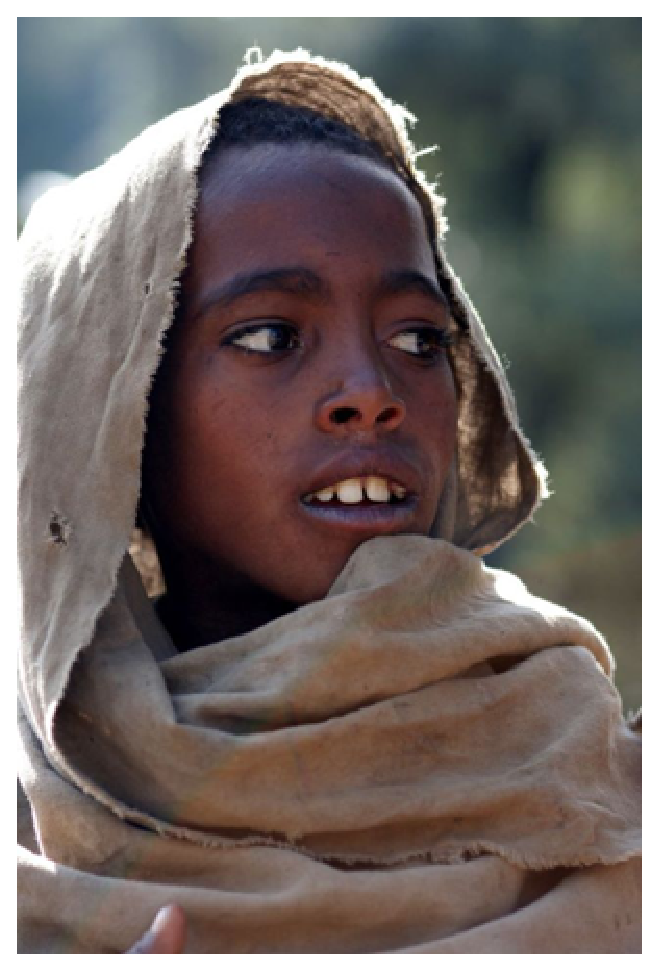
\includegraphics{etiopan.eps}}}
    \caption{Malý Etiopánek a jeho bratříček}
    \label{figure1}
\end{figure}
\newpage

Rozdíl mezi vektorovým...

\begin{figure}[h]
    \centering
    \scalebox{0.4}{
\includegraphics{oniisan.eps}}
    \caption{Vektorový obrázek}
    \label{figure2}
\end{figure}
\noindent ... a bitmapovým obrázkem
\begin{figure}[h]
    \centering
    \scalebox{0.6}{
\includegraphics{oniisan2.eps}}
    \caption{Bitmapový obrázek}
    \label{figure3}
\end{figure}

\noindent se projeví například při zvetšení.

Odkazy (nejen ty) na obrázky \ref{figure1}, \ref{figure2} a \ref{figure3}, na  
tabulky \ref{tab1} a \ref{tab2} a také na algoritmus \ref{alg1} jsou udělány pomocí 
křížových odkazů. Pak je ovšem potřeba zdrojový soubor přeložit dvakrát. \par
Vektorové obrázky lze vytvořit i přímo v {\LaTeX}u, například pomocí prostředí \texttt{picture}.
\newpage

\begin{landscape}
\begin{figure}[h]
    \centering
    \thinlines
    \setlength{\unitlength}{1mm}
    \begin{picture}(200,100)
    \put(0, 0){\framebox(200, 100){}}
    %\put(25,0){\framebox(150, 20){}}
    {\linethickness{1.5mm}\put(10,15){\line(1,0){180}}}
    %\thinlines
    \put(15,15){\framebox(50,40){}}
        \put(15,47){\line(1,0){40}}
        \put(15,19){\line(1,0){40}}
        \put(55,19){\line(0,1){28}}
    %vez
    \put(65.1,15){\framebox(15,72){}}
    %balkon
    \put(23,55.1){\framebox(3.5,20){}}
    \put(50,55.1){\framebox(3.5,20){}}
    \put(18,75.3){\framebox(47,2.5){}}
    %prava strecha
    \put(80.3,73){\line(3,-2){40}}
    \put(120.3,46.3){\line(1,0){50}}
    \put(170.3,15){\line(0,1){31.4}}
    %garaz
    \put(130,15){\framebox(33,25){}}
    \put(132,15){\framebox(29,23){}}
    %okna
    \put(87,19){\framebox(10,20){}}
    \put(105,19){\framebox(10,20){}}
    %trojuhelnikove okno
    \put(87,50){\line(0,1){10}}
    \put(87,50){\line(1,0){15}}
    \put(87,60){\line(3,-2){15}}
    %slunce
    \put(170, 85){\circle{12}}
    \end{picture}
    
    \caption{Moderní vila 21. století.}
    
    \label{landscape1}
\end{figure}
\end{landscape}




\end{document}
